\section{Installation instruction}
The game is published in the form of GitHub releases and can be downloaded from the address \url{https://github.com/Non-Euclidean-World/Hyper/releases}.
After every important improvement, a new release is shipped, so it's recommended to always download the latest version available.
A release, for example, \autoref{fig:release}, contains the following:
\begin{itemize}
    \item a ZIP archive with 64-bit Windows binaries (\texttt{win-x64}),
    \item a ZIP archive with 32-bit Windows binaries (\texttt{win-x86}),
    \item archives with the source code that the binaries were compiled from.
\end{itemize}

The application is published as \textit{self-contained} which means that it doesn't require any shared components to be installed on the target machine (even the .NET runtime).

\begin{figure}[H]
    \centering
    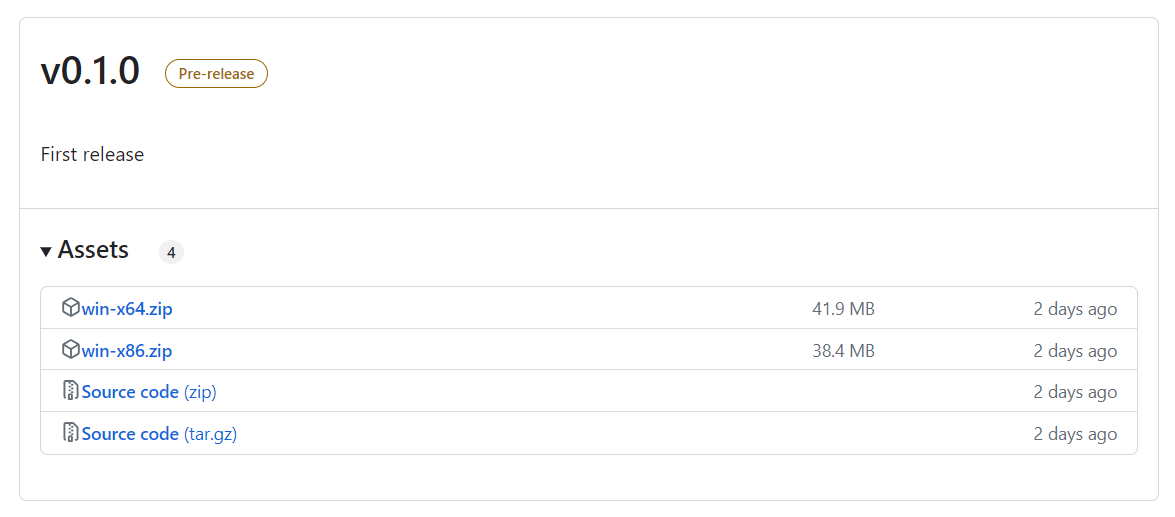
\includegraphics[width=0.8\textwidth]{sections/installation_instruction/resources/release-download.png}
    \caption{An example release}
    \label{fig:release}
\end{figure}